\chapter{Technical Foundation}

\todo{Add chapter introduction}

% In this chapter, the technical foundation of the solutions developed in this thesis is worked out. 
% Usually, this is the first chapter written by each SeniorStudent since it describes the current (technical) status 
% the further work of this thesis is based on. 
% By doing so, the continuity of the work carried out by the research group C\&M is guaranteed.
% Additionally, this chapter deals for those JuniorStudents who are co-supervised by the 
% SeniorStudent (the author of this thesis) as one of the most relevant sources for the JuniorStudents' practical work.

% Depending on the concrete topic of the thesis, the technical foundation may include the 
% (i) software and/or system architecture of the software system under investigation, 
% (ii) the artifacts relevant for the thesis, 
% (iii) tools that are applied,
% (iv) any further technical system or solution. 
% These parts of the technical foundation should be described from the viewpoint of the specific topic of this thesis. 
% For example, if an artifact is relevant for the topic, only the topic-related aspects 
% of this artifact (and not just the artifact) should be illustrated in this chapter.

% General description of concepts or solutions are NOT part of this chapter, 
% but should be transferred to other chapters of the thesis (e.g., Chapter 1 or Chapter 2). 
% This also holds for the description of concrete solutions which are NOT to be described in Chapter 5
%  but in the following chapters. The focus of Chapter 5 is to make clear what is missing in the 
% current technical solution in order to motivate the work which will be carried in this thesis 
% (and which will be further described in the following chapters).

% Relevant sources for the content of Chapter 5 are: 
% (i) WASA lecture, 
% (ii) latest Bachelor/Master/PhD theses, 
% (iii) latest publication. 
% The WASA lecture contains the current and, therefore, the ``valid version'' of concepts and solutions. 
% So this content should be trusted if there is a mismatch between WASA lecture and theses or publications.

\section{BestRentalPoC}

The BestRentalPoC is a proof of concept for the usage of decentralized identities.
BestRental is a fictive car rental company, which requires customers to have a valid driver's license
when renting a car.
For this purpose, the driving license authority can issue a customer, called Alice, a verifiable credential (VC).
The VC is stored in Alice's digital wallet.
When renting a car, Alice can present her VC to BestRental, who can then verify the validity of Alice's driver's license.

The BestRentalPoC consists of three parts: The BestRental application, the DrivingLicenseAuthority application
and the decentralized identity system.
The BestRental application allows Alice to rent a car and present her VC.
The DrivingLicenseAuthority application allows the issuance of a VC to Alice.
Finally, the decentralized identity system provides the functionality of issuing and verifying VCs.

The BestRental application consists of a browser-based frontend and a microservice, which handles the required
business logic. In the same way, the DrivingLicenseAuthority application consists of a frontend and a microservice.
Additionally, both applications have tenants in Microsoft Azure which include an Azure Active Directory and
a Key Vault called VerifiedIDVault.

The decentralized identity system consists of Microsoft Entra Verified ID and the Trust System called DidWeb.
This proof of concept utilizes Microsoft Entra Verified ID to implement decentralized identities.
Entra provides all services which are required for this. This includes services to issues and to verify VCs.

Figure \ref{fig:sps_architecture_bestrental} shows the SystemPlusSoftware Architecture of the Demonstrator BestRental.

\todo{Include latest SPS Diagram}
\begin{figure}
	\centering
	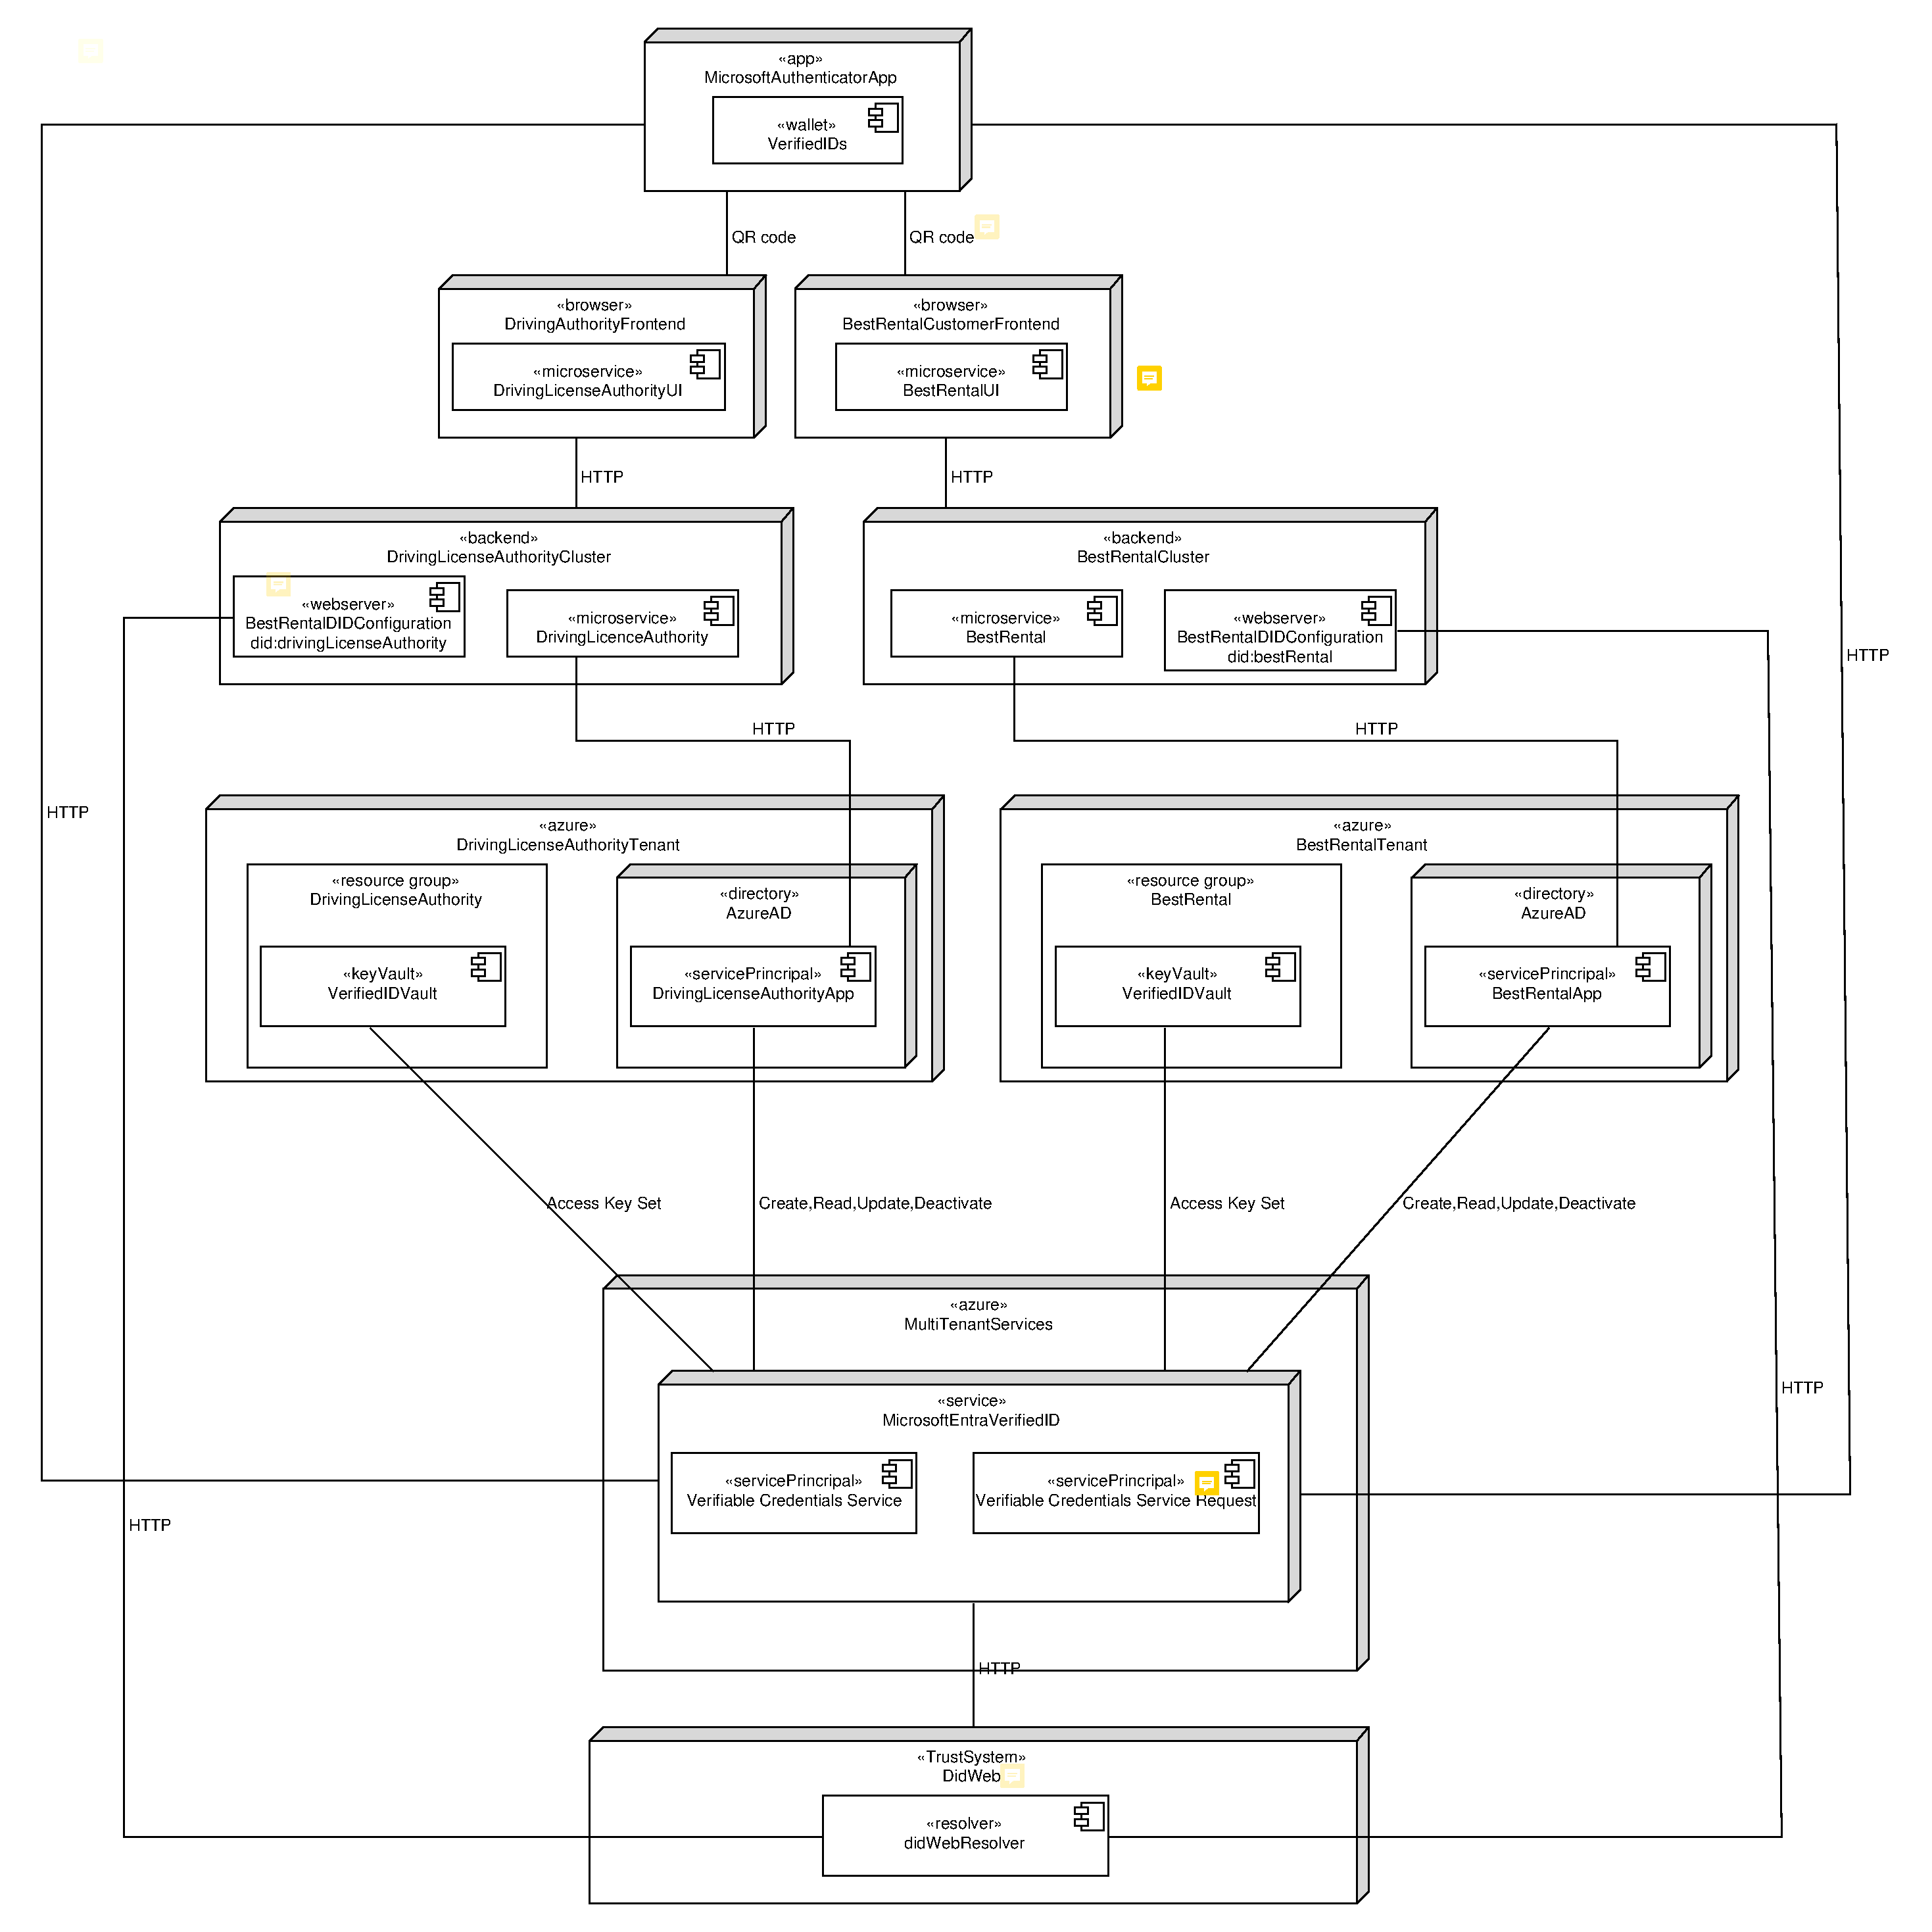
\includegraphics[width=\textwidth]{pdfs/sps_achitecture_bestrental.pdf}
	\caption{SystemPlusSoftware Architecture BestRental}
	\label{fig:sps_architecture_bestrental}
\end{figure}

\section{Decentralized Identities}

\section{Monitoring}

According to \cite{9837035}, observability consists of three pillars: Metrics, Logs, and Traces.
Metrics.
Logs are streams of textual information emitted by an application. They can contain information about important
events, like an incoming request, or provide details about the occurrence of exceptions.
Traces are a way of tracking the path of requests through a system. A trace contains detailed information
about all the services that were called during the processing of a request and can be thought of
as a stack trace for microservices.

Because of the scope of this work, only Metrics will be used. Logs and Traces will still be considered
in the development of a solution so that they may be added in the future.

Because of the scope of this work, only the pillar of Metrics is considered.

\begin{quote}
\textit{``Metrics are numerical representations of data that Ops teams use to determine the overall behavior of a system, service, or network component over time.'', \cite{9837035}}
\end{quote}

The four golden signals \cite{Beyer2016-xi}
\begin{itemize}
    \item Latency: time to service a request
    \item Traffic: requests per second
    \item Errors: rate of failed requests
    \item Saturation: how saturated are constrained resources like memory or I/O
\end{itemize}

White-box vs. Black-box Monitoring \cite{Beyer2016-xi}
\begin{itemize}
    \item White-box: Monitoring based on internal system metrics.
    \item Black-box: Monitoring based on externally visible behavior.
\end{itemize}

Internal vs. External resources in a monitoring context:
Internal resources describe resources that allow direct access to their internals.
An example of an internal resource is a self-hosted microservice.
External resources describe resources that do not allow direct access to their internals.
An example of an external resource is a Software-as-a-Service (SaaS) product which is used in a context that should be monitored.

External resources can, because of their nature, only be monitored using the Black-box approach.
Internal resources however can be monitored with both the White-box and Black-box approach.

Motivations for monitoring cloud applications \cite{6483656}
\begin{itemize}
    \item Capacity and Resource Planning
    \item Capacity and Resource Management
    \item Data Center Management
    \item SLA Management
    \item Billing
    \item Troubleshooting
    \item Performance Management
    \item Security Management
\end{itemize}

\todo{Capacity and Resource Planning}

\todo{Capacity and Resource Management}

Data Center Management is mainly concerned with the efficient usage of resources.
One key measurement of the efficiency of a data center is its energy efficiency.

SLA Management refers to the monitoring of parameters, which are defined in Service Level Agreements (SLA).
These parameters must be within set bounds for an SLA to be considered fulfilled.

Billing refers to the monitoring of parameters that influence the cost of running an application.
When an application is hosted on a cloud provider's Infrastructure-as-a-Service (IaaS) system,
one of those parameters might be the number of compute instances that an application uses.

While Troubleshooting usually refers to the tracing of requests and failures to provide a dataset for analyzing and fixing issues in an application,
Monitoring can also be used to aid in troubleshooting by recording the number of failed requests and their context.

\todo{Performance Management}

\todo{Security Management}